\documentclass[a4paper,11pt]{article}

\usepackage[T1]{fontenc}
\usepackage[utf8]{inputenc}
\usepackage[english]{babel}
\usepackage[top=3cm, left=2cm, textwidth=17cm, textheight=24cm]{geometry}
\usepackage{times}
\usepackage{multirow}
\usepackage[ruled, czech, linesnumbered, noline, longend]{algorithm2e}
\usepackage{graphics}
\usepackage{pdflscape}
\usepackage{float}


\usepackage[unicode, hidelinks]{hyperref}
\usepackage[nodayofweek]{datetime}
\usepackage[hyphenbreaks]{breakurl}
\usepackage{csquotes}
 
\begin{document}

\begin{titlepage}
    \begin{center}
        
        \Huge
        \textsc{Vysoké učení technické v~Brně}\\[0.1em]
        
        \huge
        \textsc{Fakulta~informačních technologií}
        
        \vspace*{\stretch{0.382}}
        
        \LARGE
        IMAP Client --\ Manual \\[-0.1em]

        \vspace*{\stretch{0.618}}
    \end{center}
    
    {\Large \today \hfill Tomáš Dolák}
\end{titlepage}

\newpage
\tableofcontents

\newpage
\label{firstpage}
\section{Assignment}
The project assignment in the ISA (Network Applications and Network Administration) subject was 
to create IMAP4rev1 (according to RFC3501), which will be able to communicate only over TCP/IP as well 
as using SLL/TLS - IMAPS. The following program downloads emails from the defined server in the argument 
of the program call and saves them in the output directory. If the path to the output repository 
specified by the argument does not exist, the program creates it on this path.

\section{Implementation Details}
The principles of object-oriented programming have been applied to the program code. The program is 
divided into logical classes such as the \verb!ClientConfig! class - which takes care of the configuration 
of the resulting IMAP client based on the input arguments of the program, which it also processes. 
On the result of the configuration, either an instance of the \verb!NonSecureImapClient! class is created, 
which mediates communication, classically only over TCP/IP, or an instance of the \verb!SecureImapClient! 
class, which also uses SSL/TLS in addition to TCP/IP. Both classes \verb!NonSecureImapClient! and 
\verb!SecureImapClient! inherit basic properties from \verb!BaseImapClient!, which provides features 
that are common to both derived classes, such as generating a TAG, finding the value of the current TAG or translating 
a hostname to an IPv4 address. 

\subsection{Implementation of Client}
The NonSecureImapClient and SecureClient classes are characterized by their very 
similar behavior, at the beginning when the class is instantiated they receive information 
like \verb!MailBox!, \verb!OutputDirectory!, \verb!HeadersOnly! and \verb!NewOnly! as input parameters. 
These parameters are used to define further behavior of the program and their description is given in table below.

\smallskip

\begin{center}
    \vspace{0.5cm} % Space before table
    \begin{tabular}{|c|c|}
        \hline
        \textbf{Parameter} & \textbf{Description} \\
        \hline
        MailBox & Mailbox from which emails will be downloaded \\
        \hline
        OutputDirectory & Specifies where downloaded emails will be stored \\
        \hline
        HeadersOnly & Only header of the emails will be downloaded \\
        \hline
        NewOnly & Only unseen emails will be downloaded \\
        \hline
    \end{tabular}
    \vspace{0.5cm} % Space after table
\end{center}

Then, from the user's point of view, the classes only need to call the Run method with the parameters 
server address, port login and password. This method interacts with the server and its behaviour is as follows.

\newpage
\subsection{Program Flow}
Here Will Be Description.

\begin{figure}[H]
    \centering
    \scalebox{0.5}{
        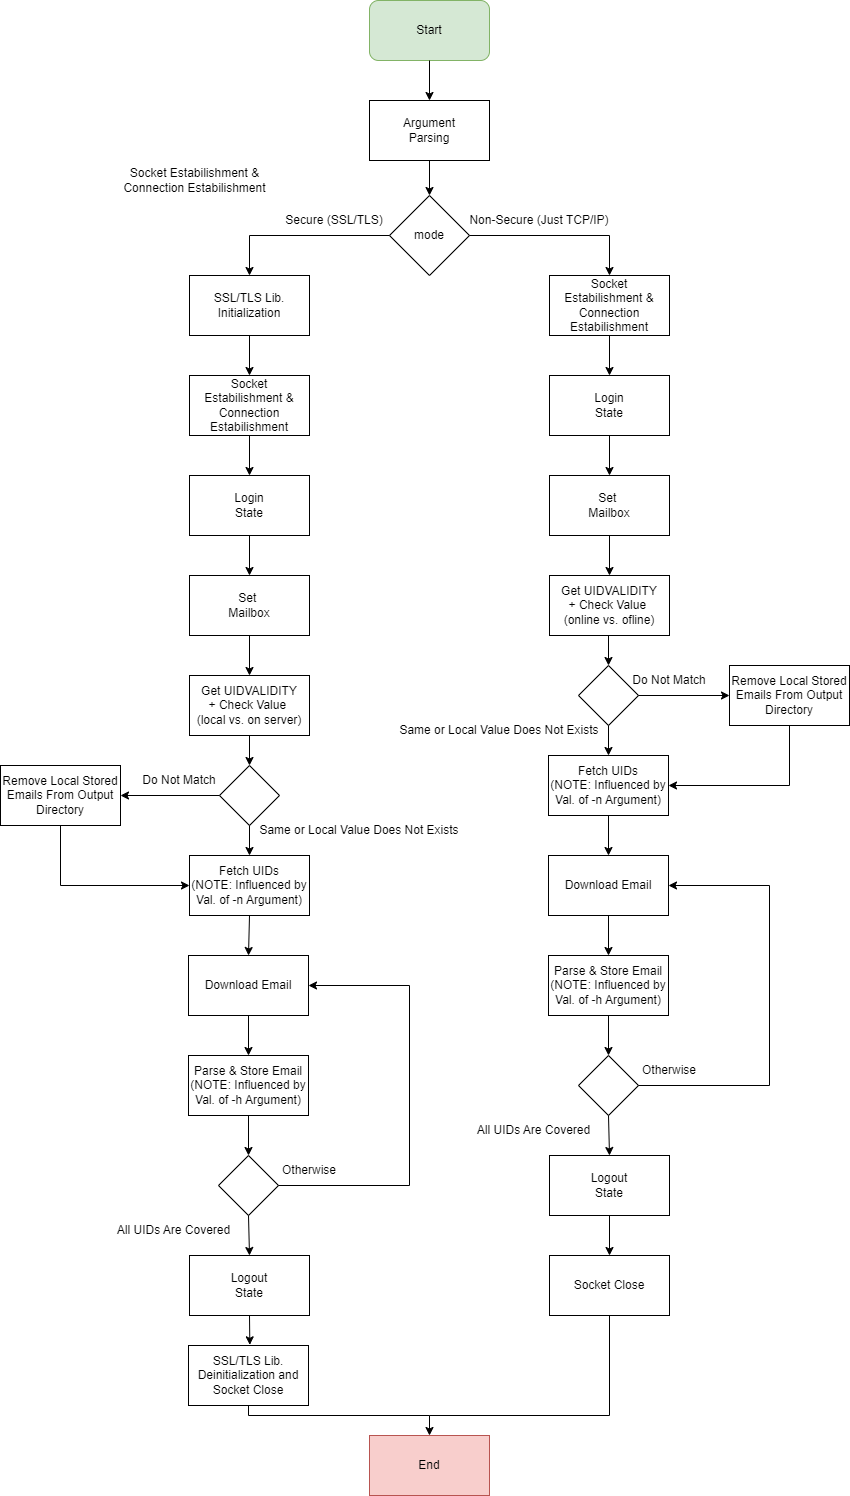
\includegraphics{program-flow-diagram.eps}
    }
    \caption{Program Flow Diagram}
    \label{figure:program-flow-diagram}
\end{figure}

\newpage
\subsection{Classes}
Here Will Be Description.

\begin{figure}[H]
    \centering
    \scalebox{0.5}{
        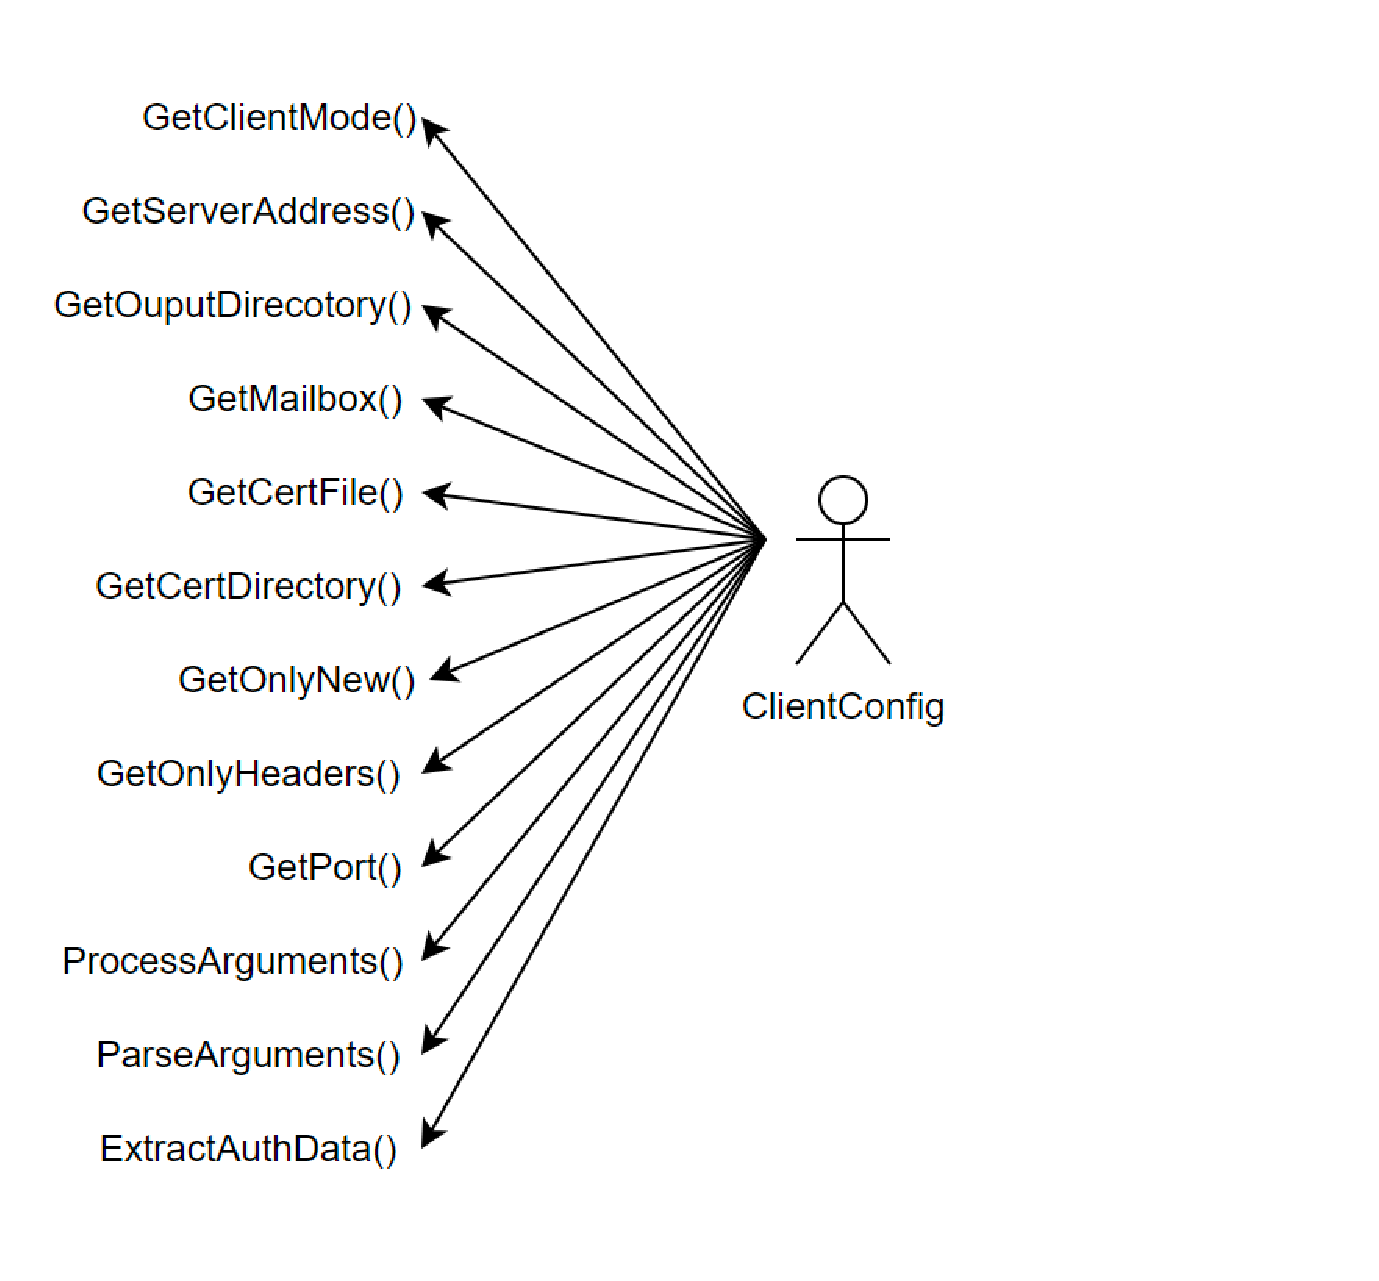
\includegraphics{ClientConfig.eps}
    }
    \caption{Program Flow Diagram}
    \label{figure:client-config}
\end{figure}

\begin{figure}[H]
    \centering
    \scalebox{0.4}{
        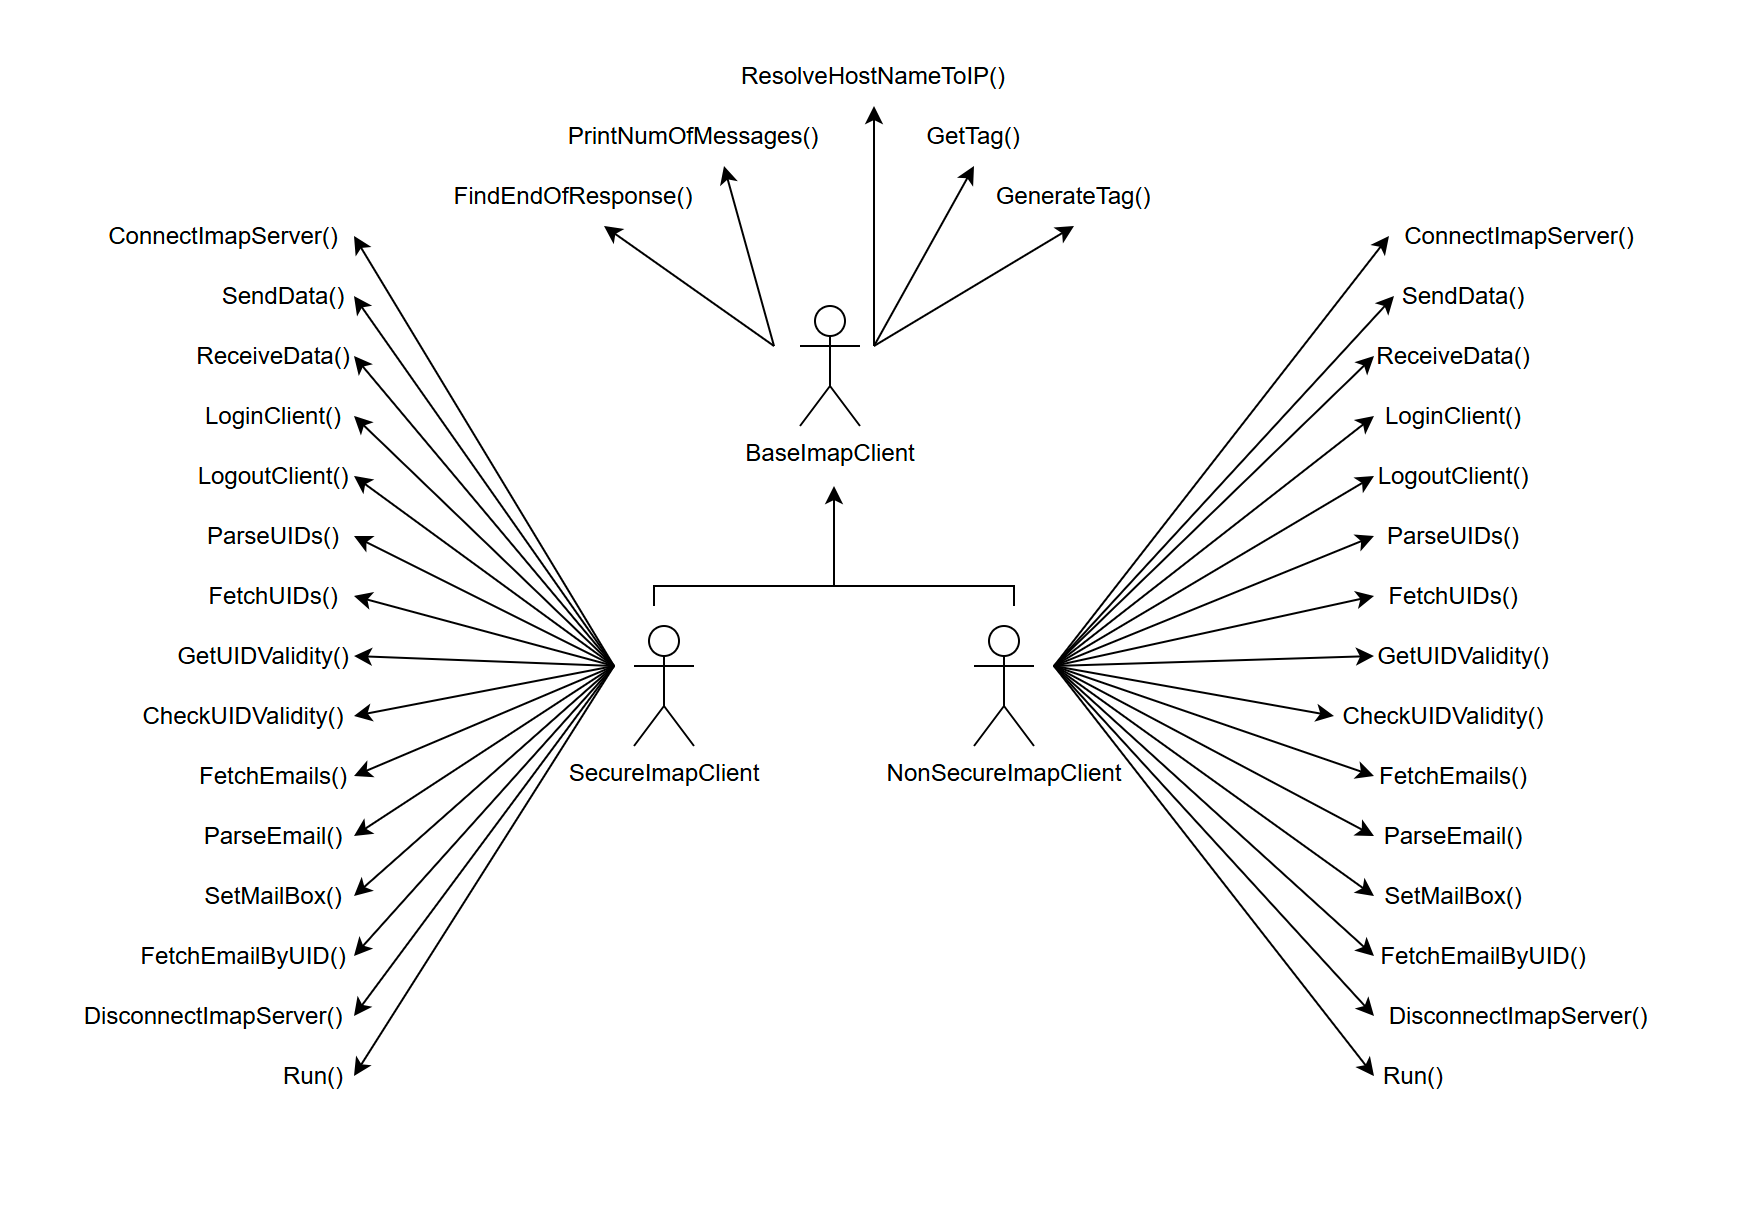
\includegraphics{ImapClient.eps}
    }
    \caption{Program Flow Diagram}
    \label{figure:imap-clients}
\end{figure}

\newpage
\section{Return Codes}
\begin{center}
    \vspace{0.5cm} % % Space before table
    \begin{tabular}{|c|c|c|}
        \hline
        \textbf{Name} & \textbf{Data Type} & \textbf{Value} \\
        \hline
        OUTPUT\_DIR\_NOT\_CREATED & int & -7 \\
        \hline
        UIDVALIDITY\_FILE\_NOT\_FOUND & int & -6 \\
        \hline
        UIDVALIDITY\_FILE\_ERROR & int & -5 \\
        \hline
        CREATE\_CONNECTION\_FAILED & int & -4 \\
        \hline
        SSL\_CERT\_VERIFICATION\_FAILED & int & -3 \\
        \hline
        FETCH\_EMAIL\_FAILED & int & -2 \\
        \hline
        SUCCESS & int & 0 \\
        \hline
        NO\_IP\_ADDR\_FOUND & int & 1 \\
        \hline
        PARSE\_ARGUMENTS\_FAILED & int & 2 \\
        \hline
        PARSE\_CREDENTIALS\_FAILED & int & 3 \\
        \hline
        SERVER\_UNKNOWN\_RESPONSE & int & 4 \\
        \hline
        TRANSMIT\_DATA\_FAILED & int & 5 \\
        \hline
        RECEIVE\_DATA\_FAILED & int & 6 \\
        \hline
        RESPONSE\_NOT\_FOUND & int & 7 \\
        \hline
        PARSE\_BY\_REGEX\_FAILED & int & 8 \\
        \hline
        NON\_UIDS\_RECEIVED & int & 9 \\
        \hline
        CONTINUE\_IN\_RECEIVING & int & 10 \\
        \hline
        UNDEFINED\_STATE & int & 11 \\
        \hline
        UID\_VALIDITY\_ERROR\_IN\_RECV & int & 14 \\
        \hline
        REMOVAL\_OF\_EMAILS\_FAILED & int & 15 \\
        \hline
        BAD\_RESPONSE & string & "Bad Response :(" \\
        \hline
    \end{tabular}
    \vspace{0.5cm} % Space after table
\end{center}


\bibliographystyle{unsrt}
\bibliography{resources}      
\end{document}
